%%%%%%%%%%%%%%%%%%%%%%%%%%%%%%%%%%%%%%%%%
% The Legrand Orange Book
% LaTeX Template
% Version 2.4 (26/09/2018)
%
% This template was downloaded from:
% http://www.LaTeXTemplates.com
%
% Original author:
% Mathias Legrand (legrand.mathias@gmail.com) with modifications by:
% Vel (vel@latextemplates.com)
%
% License:
% CC BY-NC-SA 3.0 (http://creativecommons.org/licenses/by-nc-sa/3.0/)
%
% Compiling this template:
% This template uses biber for its bibliography and makeindex for its index.
% When you first open the template, compile it from the command line with the 
% commands below to make sure your LaTeX distribution is configured correctly:
%
% 1) pdflatex main
% 2) makeindex main.idx -s StyleInd.ist
% 3) biber main
% 4) pdflatex main x 2
%
% After this, when you wish to update the bibliography/index use the appropriate
% command above and make sure to compile with pdflatex several times 
% afterwards to propagate your changes to the document.
%
% This template also uses a number of packages which may need to be
% updated to the newest versions for the template to compile. It is strongly
% recommended you update your LaTeX distribution if you have any
% compilation errors.
%
% Important note:
% Chapter heading images should have a 2:1 width:height ratio,
% e.g. 920px width and 460px height.
%
%%%%%%%%%%%%%%%%%%%%%%%%%%%%%%%%%%%%%%%%%

%----------------------------------------------------------------------------------------
%	PACKAGES AND OTHER DOCUMENT CONFIGURATIONS
%----------------------------------------------------------------------------------------

\documentclass[11pt,fleqn,oneside]{book} % Default font size and left-justified equations

%%%%%%%%%%%%%%%%%%%%%%%%%%%%%%%%%%%%%%%%%
% The Legrand Orange Book
% Structural Definitions File
% Version 2.1 (26/09/2018)
%
% Original author:
% Mathias Legrand (legrand.mathias@gmail.com) with modifications by:
% Vel (vel@latextemplates.com)
% 
% This file was downloaded from:
% http://www.LaTeXTemplates.com
%
% License:
% CC BY-NC-SA 3.0 (http://creativecommons.org/licenses/by-nc-sa/3.0/)
%
%%%%%%%%%%%%%%%%%%%%%%%%%%%%%%%%%%%%%%%%%

%----------------------------------------------------------------------------------------
%	VARIOUS REQUIRED PACKAGES AND CONFIGURATIONS
%----------------------------------------------------------------------------------------

\usepackage{graphicx} % Required for including pictures
\graphicspath{{Pictures/}} % Specifies the directory where pictures are stored

\usepackage{lipsum} % Inserts dummy text

\usepackage{tikz} % Required for drawing custom shapes

\usepackage[english]{babel} % English language/hyphenation

\usepackage{enumitem} % Customize lists
\setlist{nolistsep} % Reduce spacing between bullet points and numbered lists

\usepackage{booktabs} % Required for nicer horizontal rules in tables

\usepackage{xcolor} % Required for specifying colors by name
\definecolor{ocre}{RGB}{243,102,25} % Define the orange color used for highlighting throughout the book

\usepackage{hyperref} %hyperlinks


%----------------------------------------------------------------------------------------
%	MARGINS
%----------------------------------------------------------------------------------------

\usepackage{geometry} % Required for adjusting page dimensions and margins

\geometry{
	paper=a4paper, % Paper size, change to letterpaper for US letter size
	top=3cm, % Top margin
	bottom=3cm, % Bottom margin
	left=3cm, % Left margin
	right=3cm, % Right margin
	headheight=14pt, % Header height
	footskip=1.4cm, % Space from the bottom margin to the baseline of the footer
	headsep=10pt, % Space from the top margin to the baseline of the header
	%showframe, % Uncomment to show how the type block is set on the page
}

%----------------------------------------------------------------------------------------
%	FONTS
%----------------------------------------------------------------------------------------

\usepackage{avant} % Use the Avantgarde font for headings
%\usepackage{times} % Use the Times font for headings
\usepackage{mathptmx} % Use the Adobe Times Roman as the default text font together with math symbols from the Sym­bol, Chancery and Com­puter Modern fonts

\usepackage{microtype} % Slightly tweak font spacing for aesthetics
\usepackage[utf8]{inputenc} % Required for including letters with accents
\usepackage[T1]{fontenc} % Use 8-bit encoding that has 256 glyphs

%----------------------------------------------------------------------------------------
%	BIBLIOGRAPHY AND INDEX
%----------------------------------------------------------------------------------------

\usepackage[style=numeric,citestyle=numeric,sorting=nyt,sortcites=true,autopunct=true,babel=hyphen,hyperref=true,abbreviate=false,backref=true,backend=biber]{biblatex}
\addbibresource{bibliography.bib} % BibTeX bibliography file
\defbibheading{bibempty}{}

\usepackage{calc} % For simpler calculation - used for spacing the index letter headings correctly
\usepackage{makeidx} % Required to make an index
\makeindex % Tells LaTeX to create the files required for indexing

%----------------------------------------------------------------------------------------
%	MAIN TABLE OF CONTENTS
%----------------------------------------------------------------------------------------

\usepackage{titletoc} % Required for manipulating the table of contents

\contentsmargin{0cm} % Removes the default margin

% Part text styling (this is mostly taken care of in the PART HEADINGS section of this file)
\titlecontents{part}
	[0cm] % Left indentation
	{\addvspace{20pt}\bfseries} % Spacing and font options for parts
	{}
	{}
	{}

% Chapter text styling
\titlecontents{chapter}
	[1.25cm] % Left indentation
	{\addvspace{12pt}\large\sffamily\bfseries} % Spacing and font options for chapters
	{\color{ocre!60}\contentslabel[\Large\thecontentslabel]{1.25cm}\color{ocre}} % Formatting of numbered sections of this type
	{\color{ocre}} % Formatting of numberless sections of this type
	{\color{ocre!60}\normalsize\;\titlerule*[.5pc]{.}\;\thecontentspage} % Formatting of the filler to the right of the heading and the page number

% Section text styling
\titlecontents{section}
	[1.25cm] % Left indentation
	{\addvspace{3pt}\sffamily\bfseries} % Spacing and font options for sections
	{\contentslabel[\thecontentslabel]{1.25cm}} % Formatting of numbered sections of this type
	{} % Formatting of numberless sections of this type
	{\hfill\color{black}\thecontentspage} % Formatting of the filler to the right of the heading and the page number

% Subsection text styling
\titlecontents{subsection}
	[1.25cm] % Left indentation
	{\addvspace{1pt}\sffamily\small} % Spacing and font options for subsections
	{\contentslabel[\thecontentslabel]{1.25cm}} % Formatting of numbered sections of this type
	{} % Formatting of numberless sections of this type
	{\ \titlerule*[.5pc]{.}\;\thecontentspage} % Formatting of the filler to the right of the heading and the page number

% Figure text styling
\titlecontents{figure}
	[1.25cm] % Left indentation
	{\addvspace{1pt}\sffamily\small} % Spacing and font options for figures
	{\thecontentslabel\hspace*{1em}} % Formatting of numbered sections of this type
	{} % Formatting of numberless sections of this type
	{\ \titlerule*[.5pc]{.}\;\thecontentspage} % Formatting of the filler to the right of the heading and the page number

% Table text styling
\titlecontents{table}
	[1.25cm] % Left indentation
	{\addvspace{1pt}\sffamily\small} % Spacing and font options for tables
	{\thecontentslabel\hspace*{1em}} % Formatting of numbered sections of this type
	{} % Formatting of numberless sections of this type
	{\ \titlerule*[.5pc]{.}\;\thecontentspage} % Formatting of the filler to the right of the heading and the page number

%----------------------------------------------------------------------------------------
%	MINI TABLE OF CONTENTS IN PART HEADS
%----------------------------------------------------------------------------------------

% Chapter text styling
\titlecontents{lchapter}
	[0em] % Left indentation
	{\addvspace{15pt}\large\sffamily\bfseries} % Spacing and font options for chapters
	{\color{ocre}\contentslabel[\Large\thecontentslabel]{1.25cm}\color{ocre}} % Chapter number
	{}  
	{\color{ocre}\normalsize\sffamily\bfseries\;\titlerule*[.5pc]{.}\;\thecontentspage} % Page number

% Section text styling
\titlecontents{lsection}
	[0em] % Left indentation
	{\sffamily\small} % Spacing and font options for sections
	{\contentslabel[\thecontentslabel]{1.25cm}} % Section number
	{}
	{}

% Subsection text styling (note these aren't shown by default, display them by searchings this file for tocdepth and reading the commented text)
\titlecontents{lsubsection}
	[.5em] % Left indentation
	{\sffamily\footnotesize} % Spacing and font options for subsections
	{\contentslabel[\thecontentslabel]{1.25cm}}
	{}
	{}

%----------------------------------------------------------------------------------------
%	HEADERS AND FOOTERS
%----------------------------------------------------------------------------------------

\usepackage{fancyhdr} % Required for header and footer configuration

\pagestyle{fancy} % Enable the custom headers and footers

\renewcommand{\chaptermark}[1]{\markboth{\sffamily\normalsize\bfseries\chaptername\ \thechapter.\ #1}{}} % Styling for the current chapter in the header
\renewcommand{\sectionmark}[1]{\markright{\sffamily\normalsize\thesection\hspace{5pt}#1}{}} % Styling for the current section in the header

\fancyhf{} % Clear default headers and footers
\fancyhead[LE,RO]{\sffamily\normalsize\thepage} % Styling for the page number in the header
\fancyhead[LO]{\rightmark} % Print the nearest section name on the left side of odd pages
\fancyhead[RE]{\leftmark} % Print the current chapter name on the right side of even pages
%\fancyfoot[C]{\thepage} % Uncomment to include a footer

\renewcommand{\headrulewidth}{0.5pt} % Thickness of the rule under the header

\fancypagestyle{plain}{% Style for when a plain pagestyle is specified
	\fancyhead{}\renewcommand{\headrulewidth}{0pt}%
}

% Removes the header from odd empty pages at the end of chapters
\makeatletter
\renewcommand{\cleardoublepage}{
\clearpage\ifodd\c@page\else
\hbox{}
\vspace*{\fill}
\thispagestyle{empty}
\newpage
\fi}

%----------------------------------------------------------------------------------------
%	THEOREM STYLES
%----------------------------------------------------------------------------------------

\usepackage{amsmath,amsfonts,amssymb,amsthm} % For math equations, theorems, symbols, etc

\newcommand{\intoo}[2]{\mathopen{]}#1\,;#2\mathclose{[}}
\newcommand{\ud}{\mathop{\mathrm{{}d}}\mathopen{}}
\newcommand{\intff}[2]{\mathopen{[}#1\,;#2\mathclose{]}}
\renewcommand{\qedsymbol}{$\blacksquare$}
\newtheorem{notation}{Notation}[chapter]

% Boxed/framed environments
\newtheoremstyle{ocrenumbox}% Theorem style name
{0pt}% Space above
{0pt}% Space below
{\normalfont}% Body font
{}% Indent amount
{\small\bf\sffamily\color{ocre}}% Theorem head font
{\;}% Punctuation after theorem head
{0.25em}% Space after theorem head
{\small\sffamily\color{ocre}\thmname{#1}\nobreakspace\thmnumber{\@ifnotempty{#1}{}\@upn{#2}}% Theorem text (e.g. Theorem 2.1)
\thmnote{\nobreakspace\the\thm@notefont\sffamily\bfseries\color{black}---\nobreakspace#3.}} % Optional theorem note

\newtheoremstyle{blacknumex}% Theorem style name
{5pt}% Space above
{5pt}% Space below
{\normalfont}% Body font
{} % Indent amount
{\small\bf\sffamily}% Theorem head font
{\;}% Punctuation after theorem head
{0.25em}% Space after theorem head
{\small\sffamily{\tiny\ensuremath{\blacksquare}}\nobreakspace\thmname{#1}\nobreakspace\thmnumber{\@ifnotempty{#1}{}\@upn{#2}}% Theorem text (e.g. Theorem 2.1)
\thmnote{\nobreakspace\the\thm@notefont\sffamily\bfseries---\nobreakspace#3.}}% Optional theorem note

\newtheoremstyle{blacknumbox} % Theorem style name
{0pt}% Space above
{0pt}% Space below
{\normalfont}% Body font
{}% Indent amount
{\small\bf\sffamily}% Theorem head font
{\;}% Punctuation after theorem head
{0.25em}% Space after theorem head
{\small\sffamily\thmname{#1}\nobreakspace\thmnumber{\@ifnotempty{#1}{}\@upn{#2}}% Theorem text (e.g. Theorem 2.1)
\thmnote{\nobreakspace\the\thm@notefont\sffamily\bfseries---\nobreakspace#3.}}% Optional theorem note

% Non-boxed/non-framed environments
\newtheoremstyle{ocrenum}% Theorem style name
{5pt}% Space above
{5pt}% Space below
{\normalfont}% Body font
{}% Indent amount
{\small\bf\sffamily\color{ocre}}% Theorem head font
{\;}% Punctuation after theorem head
{0.25em}% Space after theorem head
{\small\sffamily\color{ocre}\thmname{#1}\nobreakspace\thmnumber{\@ifnotempty{#1}{}\@upn{#2}}% Theorem text (e.g. Theorem 2.1)
\thmnote{\nobreakspace\the\thm@notefont\sffamily\bfseries\color{black}---\nobreakspace#3.}} % Optional theorem note
\makeatother

% Defines the theorem text style for each type of theorem to one of the three styles above
\newcounter{dummy} 
\numberwithin{dummy}{section}
\theoremstyle{ocrenumbox}
\newtheorem{theoremeT}[dummy]{Theorem}
\newtheorem{problem}{Problem}[chapter]
\newtheorem{exerciseT}{Exercise}[chapter]
\theoremstyle{blacknumex}
\newtheorem{exampleT}{Example}[chapter]
\theoremstyle{blacknumbox}
\newtheorem{vocabulary}{Vocabulary}[chapter]
\newtheorem{definitionT}{Definition}[section]
\newtheorem{corollaryT}[dummy]{Corollary}
\theoremstyle{ocrenum}
\newtheorem{proposition}[dummy]{Proposition}

%----------------------------------------------------------------------------------------
%	DEFINITION OF COLORED BOXES
%----------------------------------------------------------------------------------------

\RequirePackage[framemethod=default]{mdframed} % Required for creating the theorem, definition, exercise and corollary boxes

% Theorem box
\newmdenv[skipabove=7pt,
skipbelow=7pt,
backgroundcolor=black!5,
linecolor=ocre,
innerleftmargin=5pt,
innerrightmargin=5pt,
innertopmargin=5pt,
leftmargin=0cm,
rightmargin=0cm,
innerbottommargin=5pt]{tBox}

% Exercise box	  
\newmdenv[skipabove=7pt,
skipbelow=7pt,
rightline=false,
leftline=true,
topline=false,
bottomline=false,
backgroundcolor=ocre!10,
linecolor=ocre,
innerleftmargin=5pt,
innerrightmargin=5pt,
innertopmargin=5pt,
innerbottommargin=5pt,
leftmargin=0cm,
rightmargin=0cm,
linewidth=4pt]{eBox}	

% Definition box
\newmdenv[skipabove=7pt,
skipbelow=7pt,
rightline=false,
leftline=true,
topline=false,
bottomline=false,
linecolor=ocre,
innerleftmargin=5pt,
innerrightmargin=5pt,
innertopmargin=0pt,
leftmargin=0cm,
rightmargin=0cm,
linewidth=4pt,
innerbottommargin=0pt]{dBox}	

% Corollary box
\newmdenv[skipabove=7pt,
skipbelow=7pt,
rightline=false,
leftline=true,
topline=false,
bottomline=false,
linecolor=gray,
backgroundcolor=black!5,
innerleftmargin=5pt,
innerrightmargin=5pt,
innertopmargin=5pt,
leftmargin=0cm,
rightmargin=0cm,
linewidth=4pt,
innerbottommargin=5pt]{cBox}

% Creates an environment for each type of theorem and assigns it a theorem text style from the "Theorem Styles" section above and a colored box from above
\newenvironment{theorem}{\begin{tBox}\begin{theoremeT}}{\end{theoremeT}\end{tBox}}
\newenvironment{exercise}{\begin{eBox}\begin{exerciseT}}{\hfill{\color{ocre}\tiny\ensuremath{\blacksquare}}\end{exerciseT}\end{eBox}}				  
\newenvironment{definition}{\begin{dBox}\begin{definitionT}}{\end{definitionT}\end{dBox}}	
\newenvironment{example}{\begin{exampleT}}{\hfill{\tiny\ensuremath{\blacksquare}}\end{exampleT}}		
\newenvironment{corollary}{\begin{cBox}\begin{corollaryT}}{\end{corollaryT}\end{cBox}}	

%----------------------------------------------------------------------------------------
%	REMARK ENVIRONMENT
%----------------------------------------------------------------------------------------

\newenvironment{remark}{\par\vspace{10pt}\small % Vertical white space above the remark and smaller font size
\begin{list}{}{
\leftmargin=35pt % Indentation on the left
\rightmargin=25pt}\item\ignorespaces % Indentation on the right
\makebox[-2.5pt]{\begin{tikzpicture}[overlay]
\node[draw=ocre!60,line width=1pt,circle,fill=ocre!25,font=\sffamily\bfseries,inner sep=2pt,outer sep=0pt] at (-15pt,0pt){\textcolor{ocre}{R}};\end{tikzpicture}} % Orange R in a circle
\advance\baselineskip -1pt}{\end{list}\vskip5pt} % Tighter line spacing and white space after remark

%----------------------------------------------------------------------------------------
%	SECTION NUMBERING IN THE MARGIN
%----------------------------------------------------------------------------------------

\makeatletter
\renewcommand{\@seccntformat}[1]{\llap{\textcolor{ocre}{\csname the#1\endcsname}\hspace{1em}}}                    
\renewcommand{\section}{\@startsection{section}{1}{\z@}
{-4ex \@plus -1ex \@minus -.4ex}
{1ex \@plus.2ex }
{\normalfont\large\sffamily\bfseries}}
\renewcommand{\subsection}{\@startsection {subsection}{2}{\z@}
{-3ex \@plus -0.1ex \@minus -.4ex}
{0.5ex \@plus.2ex }
{\normalfont\sffamily\bfseries}}
\renewcommand{\subsubsection}{\@startsection {subsubsection}{3}{\z@}
{-2ex \@plus -0.1ex \@minus -.2ex}
{.2ex \@plus.2ex }
{\normalfont\small\sffamily\bfseries}}                        
\renewcommand\paragraph{\@startsection{paragraph}{4}{\z@}
{-2ex \@plus-.2ex \@minus .2ex}
{.1ex}
{\normalfont\small\sffamily\bfseries}}

%----------------------------------------------------------------------------------------
%	PART HEADINGS
%----------------------------------------------------------------------------------------

% Numbered part in the table of contents
\newcommand{\@mypartnumtocformat}[2]{%
	\setlength\fboxsep{0pt}%
	\noindent\colorbox{ocre!20}{\strut\parbox[c][.7cm]{\ecart}{\color{ocre!70}\Large\sffamily\bfseries\centering#1}}\hskip\esp\colorbox{ocre!40}{\strut\parbox[c][.7cm]{\linewidth-\ecart-\esp}{\Large\sffamily\centering#2}}%
}

% Unnumbered part in the table of contents
\newcommand{\@myparttocformat}[1]{%
	\setlength\fboxsep{0pt}%
	\noindent\colorbox{ocre!40}{\strut\parbox[c][.7cm]{\linewidth}{\Large\sffamily\centering#1}}%
}

\newlength\esp
\setlength\esp{4pt}
\newlength\ecart
\setlength\ecart{1.2cm-\esp}
\newcommand{\thepartimage}{}%
\newcommand{\partimage}[1]{\renewcommand{\thepartimage}{#1}}%
\def\@part[#1]#2{%
\ifnum \c@secnumdepth >-2\relax%
\refstepcounter{part}%
\addcontentsline{toc}{part}{\texorpdfstring{\protect\@mypartnumtocformat{\thepart}{#1}}{\partname~\thepart\ ---\ #1}}
\else%
\addcontentsline{toc}{part}{\texorpdfstring{\protect\@myparttocformat{#1}}{#1}}%
\fi%
\startcontents%
\markboth{}{}%
{\thispagestyle{empty}%
\begin{tikzpicture}[remember picture,overlay]%
\node at (current page.north west){\begin{tikzpicture}[remember picture,overlay]%	
\fill[ocre!20](0cm,0cm) rectangle (\paperwidth,-\paperheight);
\node[anchor=north] at (4cm,-3.25cm){\color{ocre!40}\fontsize{220}{100}\sffamily\bfseries\thepart}; 
\node[anchor=south east] at (\paperwidth-1cm,-\paperheight+1cm){\parbox[t][][t]{8.5cm}{
\printcontents{l}{0}{\setcounter{tocdepth}{1}}% The depth to which the Part mini table of contents displays headings; 0 for chapters only, 1 for chapters and sections and 2 for chapters, sections and subsections
}};
\node[anchor=north east] at (\paperwidth-1.5cm,-3.25cm){\parbox[t][][t]{15cm}{\strut\raggedleft\color{white}\fontsize{30}{30}\sffamily\bfseries#2}};
\end{tikzpicture}};
\end{tikzpicture}}%
\@endpart}
\def\@spart#1{%
\startcontents%
\phantomsection
{\thispagestyle{empty}%
\begin{tikzpicture}[remember picture,overlay]%
\node at (current page.north west){\begin{tikzpicture}[remember picture,overlay]%	
\fill[ocre!20](0cm,0cm) rectangle (\paperwidth,-\paperheight);
\node[anchor=north east] at (\paperwidth-1.5cm,-3.25cm){\parbox[t][][t]{15cm}{\strut\raggedleft\color{white}\fontsize{30}{30}\sffamily\bfseries#1}};
\end{tikzpicture}};
\end{tikzpicture}}
\addcontentsline{toc}{part}{\texorpdfstring{%
\setlength\fboxsep{0pt}%
\noindent\protect\colorbox{ocre!40}{\strut\protect\parbox[c][.7cm]{\linewidth}{\Large\sffamily\protect\centering #1\quad\mbox{}}}}{#1}}%
\@endpart}
\def\@endpart{\vfil\newpage
\if@twoside
\if@openright
\null
\thispagestyle{empty}%
\newpage
\fi
\fi
\if@tempswa
\twocolumn
\fi}

%----------------------------------------------------------------------------------------
%	CHAPTER HEADINGS
%----------------------------------------------------------------------------------------

% A switch to conditionally include a picture, implemented by Christian Hupfer
\newif\ifusechapterimage
\usechapterimagetrue
\newcommand{\thechapterimage}{}%
\newcommand{\chapterimage}[1]{\ifusechapterimage\renewcommand{\thechapterimage}{#1}\fi}%
\newcommand{\autodot}{.}
\def\@makechapterhead#1{%
{\parindent \z@ \raggedright \normalfont
\ifnum \c@secnumdepth >\m@ne
\if@mainmatter
\begin{tikzpicture}[remember picture,overlay]
\node at (current page.north west)
{\begin{tikzpicture}[remember picture,overlay]
\node[anchor=north west,inner sep=0pt] at (0,0) {\ifusechapterimage\includegraphics[width=\paperwidth]{\thechapterimage}\fi};
\draw[anchor=west] (\Gm@lmargin,-9cm) node [line width=2pt,rounded corners=15pt,draw=ocre,fill=white,fill opacity=0.5,inner sep=15pt]{\strut\makebox[22cm]{}};
\draw[anchor=west] (\Gm@lmargin+.3cm,-9cm) node {\huge\sffamily\bfseries\color{black}\thechapter\autodot~#1\strut};
\end{tikzpicture}};
\end{tikzpicture}
\else
\begin{tikzpicture}[remember picture,overlay]
\node at (current page.north west)
{\begin{tikzpicture}[remember picture,overlay]
\node[anchor=north west,inner sep=0pt] at (0,0) {\ifusechapterimage\includegraphics[width=\paperwidth]{\thechapterimage}\fi};
\draw[anchor=west] (\Gm@lmargin,-9cm) node [line width=2pt,rounded corners=15pt,draw=ocre,fill=white,fill opacity=0.5,inner sep=15pt]{\strut\makebox[22cm]{}};
\draw[anchor=west] (\Gm@lmargin+.3cm,-9cm) node {\huge\sffamily\bfseries\color{black}#1\strut};
\end{tikzpicture}};
\end{tikzpicture}
\fi\fi\par\vspace*{270\p@}}}

%-------------------------------------------

\def\@makeschapterhead#1{%
\begin{tikzpicture}[remember picture,overlay]
\node at (current page.north west)
{\begin{tikzpicture}[remember picture,overlay]
\node[anchor=north west,inner sep=0pt] at (0,0) {\ifusechapterimage\includegraphics[width=\paperwidth]{\thechapterimage}\fi};
\draw[anchor=west] (\Gm@lmargin,-9cm) node [line width=2pt,rounded corners=15pt,draw=ocre,fill=white,fill opacity=0.5,inner sep=15pt]{\strut\makebox[22cm]{}};
\draw[anchor=west] (\Gm@lmargin+.3cm,-9cm) node {\huge\sffamily\bfseries\color{black}#1\strut};
\end{tikzpicture}};
\end{tikzpicture}
\par\vspace*{270\p@}}
\makeatother

%----------------------------------------------------------------------------------------
%	LINKS
%----------------------------------------------------------------------------------------

\usepackage{hyperref}
\hypersetup{hidelinks,backref=true,pagebackref=true,hyperindex=true,colorlinks=false,breaklinks=true,urlcolor=ocre,bookmarks=true,bookmarksopen=false}

\usepackage{bookmark}
\bookmarksetup{
open,
numbered,
addtohook={%
\ifnum\bookmarkget{level}=0 % chapter
\bookmarksetup{bold}%
\fi
\ifnum\bookmarkget{level}=-1 % part
\bookmarksetup{color=ocre,bold}%
\fi
}
}
 % Insert the commands.tex file which contains the majority of the structure behind the template

%\hypersetup{pdftitle={Title},pdfauthor={Author}} % Uncomment and fill out to include PDF metadata for the author and title of the book

%----------------------------------------------------------------------------------------

\begin{document}

%----------------------------------------------------------------------------------------
%	TITLE PAGE
%----------------------------------------------------------------------------------------

\begingroup
\thispagestyle{empty} % Suppress headers and footers on the title page
\begin{tikzpicture}[remember picture,overlay]
\node[inner sep=0pt] (background) at (current page.center) {
\includegraphics[width=\paperwidth]{background.pdf}};
\draw (current page.center) node [fill=ocre!30!white,fill opacity=0.6,text opacity=1,inner sep=1cm]{\Huge\centering\bfseries\sffamily\parbox[c][][t]{\paperwidth}{\centering Quick Survival Guide\\for CS \& Networking students\\[15pt] % Book title
{\Large Guidelines for a good journey in Pisa}\\[20pt] % Subtitle
{\huge by: D.Gadler, F.Tosoni, N.Tonci, L.Di Gregorio Zitella, T.Mustafa}}}; % Author name
\end{tikzpicture}
\vfill
\endgroup

%----------------------------------------------------------------------------------------
%	COPYRIGHT PAGE
%----------------------------------------------------------------------------------------

\newpage
~\vfill
\thispagestyle{empty}

\noindent Copyright \copyright\ 2019 University of Pisa\\ % Copyright notice

%\noindent \textsc{Published by Someone}\\ % Publisher

%\noindent \textsc{book-website.com}\\ % URL

%\noindent Licensed under the Creative Commons Attribution-NonCommercial 3.0 Unported License (the ``License''). You may not use this file except in compliance with the License. You may obtain a copy of the License at \url{http://creativecommons.org/licenses/by-nc/3.0}. Unless required by applicable law or agreed to in writing, software distributed under the License is distributed on an \textsc{``as is'' basis, without warranties or conditions of any kind}, either express or implied. See the License for the specific language governing permissions and limitations under the License.\\ % License information, replace this with your own license (if any)

\noindent \textit{First edition, March 2019} % Printing/edition date

%----------------------------------------------------------------------------------------
%	TABLE OF CONTENTS
%----------------------------------------------------------------------------------------

%\usechapterimagefalse % If you don't want to include a chapter image, use this to toggle images off - it can be enabled later with \usechapterimagetrue

\chapterimage{pisa.jpg} % Table of contents heading image

\pagestyle{empty} % Disable headers and footers for the following pages

\tableofcontents % Print the table of contents itself

\cleardoublepage % Forces the first chapter to start on an odd page so it's on the right side of the book

\pagestyle{fancy} % Enable headers and footers again

%----------------------------------------------------------------------------------------
%	CHAPTER 
%----------------------------------------------------------------------------------------

\chapterimage{intro.png} % Chapter heading image

\chapter{Introduction}

%------------------------------------------------

\section{Welcome!}\index{Welcome!}

Dear new student of the Master’s in Computer Science and Networking,
Firstly, congratulations on being admitted!  This guide was born from the idea of providing new students of the Master’s in Computer Science and Networking at Scuola Superiore Sant’Anna and at the University of Pisa with all the information needed for a kick-start into this study course. We representatives personally felt a bit “lost” at the very beginning of our Master’s and it was not always easy to find all information needed for a smooth beginning of our Master’s (just as an example: to find out if we were entitled to use the Sant’Anna mensa, we had to go through three different secretaries, and same thing with the Sant’Anna library. Such piece of information is not written on any website!) 
We hope to make a good favour to new students of the Master’s in Computer Science and networking by compounding in a single place all relevant information for a brilliant start!

%------------------------------------------------

\section{Master’s Courses organization}\index{Master’s Courses organization}

The Master’s in Computer Science and networking is a two-year study program. Generally, the first year is somewhat “tougher”, as you will be exposed to subjects very different from one another offered at different departments. You will also need to get accustomed  to the courses’ structuring and you will need to find your own method to cope with the demanding study load. However, if you manage to manage to pass all first-year exams on time, you will have developed very good hard-working and organizational skills. Furthermore, first-year courses are more theoretical than second-year courses, in general.  This is a very characteristic of our Master’s: it provides students with a very solid theoretical background during the first year, then each one of us is left free to specialize in their own field of interest. 
Trust me, it is highly \textbf{NOT RECOMMENDED} to take second-year courses before passing first-year courses, because 2nd-year courses often leverage the theoretical knowledge you acquired during the first year (e.g. it is very useful to know about the Map-Reduce paradigm from a theoretical point of view before studying a framework implementing it). 

%----------------------------------------------------------------------------------------
%	CHAPTER 
%----------------------------------------------------------------------------------------

\chapterimage{enrollment.png} % Chapter heading image

\chapter{Enrollment}

%------------------------------------------------

\section{Secretary Office}\index{Secretary Office}

Upon arriving in Pisa,and possibly before lectures begin, you will have to enroll at the University of Pisa at the “Segreteria Studenti” of the Polo Fibonacci in Largo Bruno Pontecorvo 3. It may be very crowded upon beginning of the lectures’ period, so it is highly recommended to go there as soon as it opens. Remember to bring all the documents listed in your enrollment invitation, and ask for “Signora Bigi”. She is the only one that knows something there about our Master’s, whereas.
The student secretary will hand you the Student booklet (libretto dello studente), which you will need for registering an exam once you accept an exam’s grade and the Student card, which you can use for paying in any university mensa of Tuscany. The student secretary is your contact point for everything that concerns university taxes and grades’ registration (e.g. I once had to go there for having a grade registered manually, as the professor could not do it because of a bug in the system). 

\begin{figure}[h]
    \centering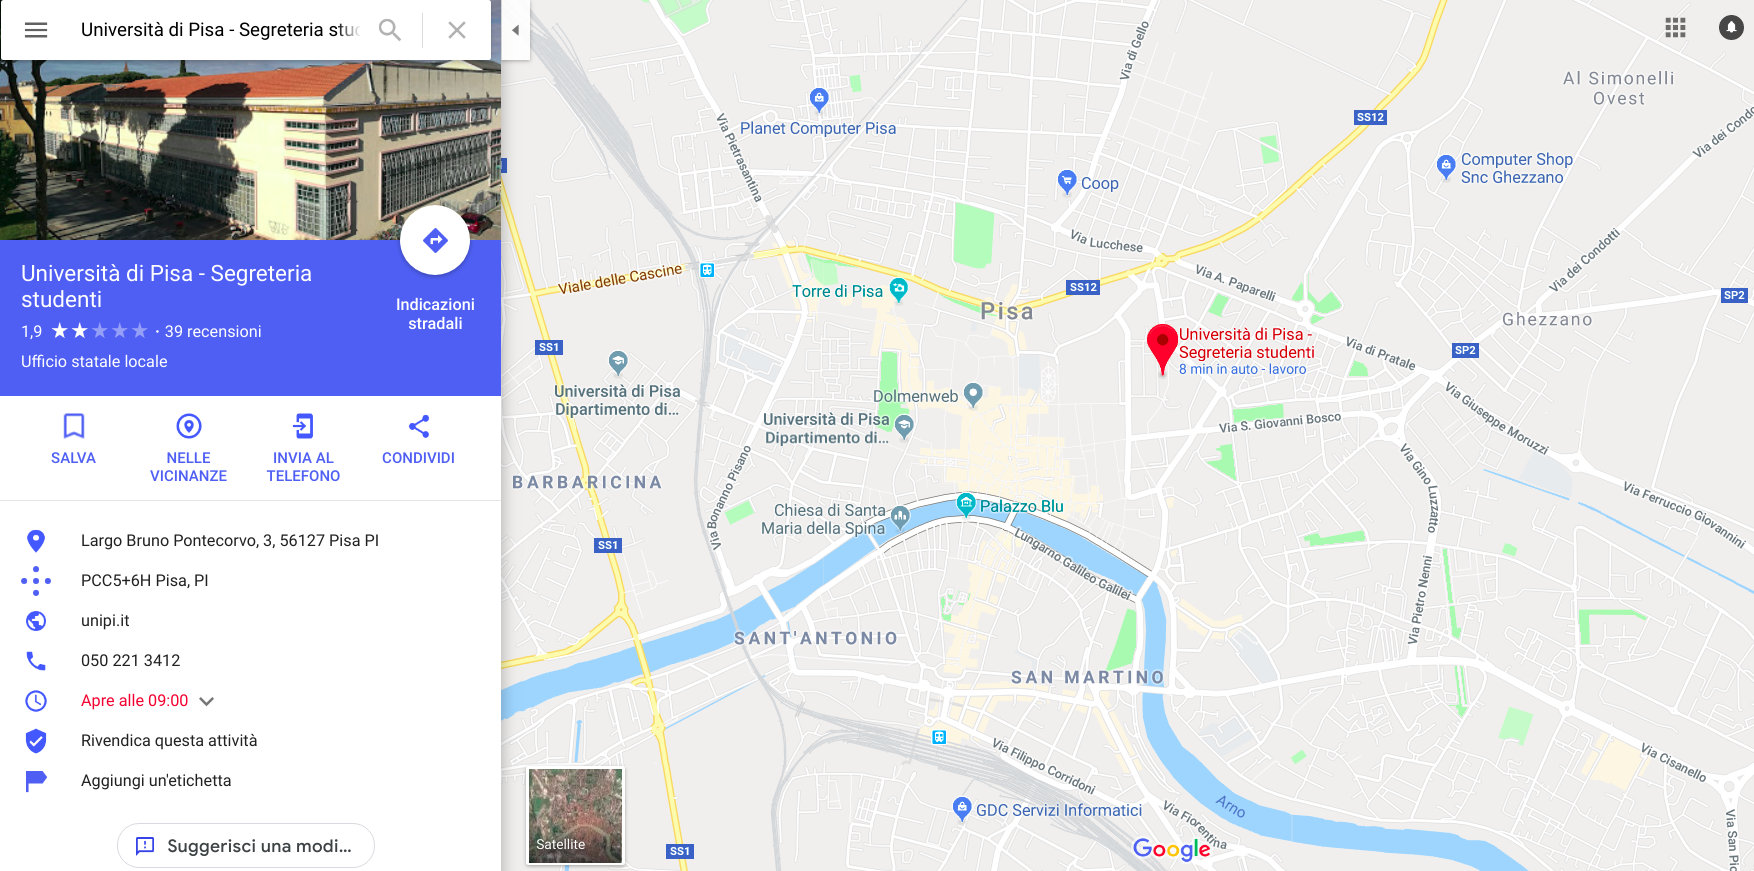
\includegraphics[width=\linewidth]{segreteria.png}
    \caption{Location of the Student Secretery. Opening hours: 9-12 AM. Monday-friday}
\end{figure}

%----------------------------------------------------------------------------------------
%	CHAPTER 
%----------------------------------------------------------------------------------------

\chapterimage{scrooge.png} % Chapter heading image

\chapter{Scolarships and Awards}

%------------------------------------------------

\section{International Students’ Scholarships}\index{International Students’ Scholarships}
TODO

\section{Need-Based Scholarships}
The DSU provides need-based scholarships for all students meeting the requirements set by the DSU. This involved your family’s economical condition and, starting from the second year, the amount of exams passed. For all official information, please refer to the official DSU website: https://portale.dsu.toscana.it/

\section{Merit-based Study Awards}\index{Merit-based Study Awards}
Currently, about 3-4 awards are assigned yearly to the students having passed the highest amount of exams before October 1 of the following year for an amount of EUR 2000 each. In case of tie on the amount of CFUs, the award is assigned to the student with the highest GPA. For the exact amount of awards and the value of the scholarship, please refer to the official call published each year around the end of July. Merit study awards are taxed by 25\% IRPEF as by the time of writing. So, if you  won a EUR 2000 scholarship, you would actually get EUR 1500 in practice. 
Minimum Requirements: 45 CFU and 27/30 GPA
So, studying hard is worth it not just for your own personal convenience, but also from an economical point of view ;-). You can get this award even if you got the DSU scholarship or the international students’ scholarship. 


%----------------------------------------------------------------------------------------
%	CHAPTER 
%----------------------------------------------------------------------------------------

\chapterimage{sssup.jpg} % Chapter heading image

\chapter{Sant'Anna Services}

%------------------------------------------------

\section{Badge}\index{Badge}
At the beginning of the academic year, usually around the beginning of October, you will be provided with: a Sant’Anna Badge, a Sant’Anna shopping bag, a Sant’Anna guest account for printing in the central library and a TeCIP account for printing at the TeCIP institute. 

%------------------------------------------------

\section{Others}\index{Others}
Currently, we are entitled to the following services from Scuola Superiore Sant’Anna:
\begin{itemize}
\item Sant’Anna Mensa in the central Sant’Anna building in Piazza Martiri della Libertà at the cost of: EUR 6.29 for a full meal, EUR 4.2 for a half-meal. It’s not very convenient wrt. DSU canteens, but for further information, please refer to the official Sant’Anna mensa website: http://www.sssupmensa.it/
Opening hours: 
\item Free Coffee: We are allowed to get free coffee at the Sant’Anna mensa during the mensa opening hours at the automatic machine just at the entrance. 
\item 2000 free photocopies per year at the TeCIP: you are allowed to use the printer at the entrance of the TeCIP both for scanning and printing up to 2000 pages per year with recycled paper by using an 8-digit account you are provided by the TeCIP didactic secretary. These 2000 copies are renewed on December 1 of every year. 
How to print: Bring a USB stick formatted in FAT32 format, or format the USB stick at the printer itself, then put the file. NB: It only supports printing of PDF format files either in one-sided or two-sided way, so make sure your files are in the right format before printing. 
\item EUR 50 printing credit per year at the Central Library: You are entitled to EUR 50 credit to. Printing a single sheet costs EUR 0.05, so that makes 1000 copies. This is not recycled paper, so print with more care than I do. Again, this EUR 50 credit is renewed every year on December 1. 
How to print: Log into the computers at the Sant’Anna library with your Sant’Anna guest account, starting with gxxx, then submit a print job by going to File $\rightarrow$ Print $\rightarrow$ Xerox or HP Laserjet printer. You may print files in any format, as they will be converted to PDF automatically when you submit the print job. 
\item Usage of the Central library in the standard opening hours: You may use the central library in Piazza Martiti della Libertà during the standard opening hours. Outside the opening hours, you may still stay in the library, but you won’t be able to open the front door without an enabled badge. For further information: https://www.santannapisa.it/it/biblioteca
Opening hours:  from 8.00 to 18.00. Monday – Friday. 
\item Usage of the Computers at TeCIP: You may use the computers in the PC Room at the TeCIP that currently run Linux. Use the password: master
\item Usage of the Wi-Fi: You may use the “Scuola Superiore Sant’Anna” Wi-Fi Network by entering your guest username and password.
\item Sant’Anna Language courses: You are theoretically allowed to attend Sant’Anna italian language courses for free if you would like to attend. For further information, ask the central secretary at the main Sant’Anna building in Piazza Martiri della Libertà. 
\end{itemize}

%----------------------------------------------------------------------------------------
%	CHAPTER 
%----------------------------------------------------------------------------------------

\chapterimage{CNRPISA.jpg} % Chapter heading image

\chapter{CNR Services}

%-----------------------------------------------

\section{Mensa}\index{Mensa}
Theoretically, we are allowed to use the mensa at the CNR with the Sant’Anna card, although I do not know how much this costs or whether one can also pay cash. I will try to get more information in the next weeks as I’m about to start working on my thesis there

%-----------------------------------------------

\section{Scientific Library}\index{Scientific Library}
We are allowed to use the CNR library close to the Sant’Anna building at the CNR Research area.

For further information, refer to the official library website: \url{http://library.isti.cnr.it/index.php/it/}.
Opening hours are 8.30 – 19.30. Monday to Friday.

%----------------------------------------------------------------------------------------
%	CHAPTER 
%----------------------------------------------------------------------------------------

\chapterimage{polo-fibonacci.png} % Chapter heading image

\chapter{UniPi Services}

%-----------------------------------------------

\section{GAP}\index{GAP}
GAP stands for ``Room Managment Pisa'' and is avilable as bot on telegram. When instructed it reveales current empty rooms in whatever department around the city: very useful when you are looking for a peaceful place to start studying!
\begin{figure}[h]
  \centering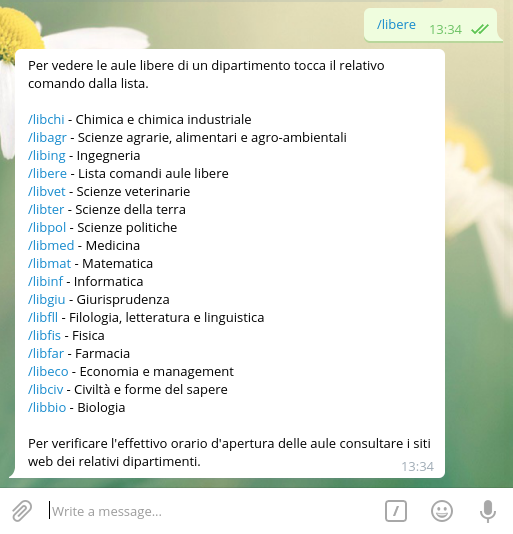
\includegraphics[width=\linewidth]{gap.png}
  \caption{GAP provides diffrent commands that allow you to find empty rooms in Pisa in every UniPi department.}
\end{figure}

%-----------------------------------------------

\Section{Software}
\begin{itemize}
  \item Microsoft Office 365 license, online Microsoft Office 365. You have Linux and cannot install Microsoft office? Unipi lets you use Microsoft Office 365 online
  \item \textsc{Matlab} is also available under a license for academic use on a maximum number of 4 machines. Visit the site: \url{http://doc.sid.unipi.it/Campus_Matlab}
\end{itemize}  

\section{UniPi Services}
The University of Pisa offers several different services to its students. I would like to summarize the most important ones as follows:
\item Libraries all around the city.
\item 5 Canteens around the city, both for lunch and dinner at a convenient cost (see Figure \ref{fig:mense}).
\item CUS Pisa: sport activities and sport tournaments of any kind all around the year. Web site: \url{http://cuspisa.unipi.it/index.php/corsi-e-tornei.html}. You may attend tennis, swimming, kung-fu courses, just to mention a few. You may also book a football field for 55 EUR an hour including lightning (slightly less than 5.5 EUR each, if you play 5 vs 5).
If you want to attend a sport course, you will need a “certificato medico”, which you can get from an ASL doctor in Pisa for 20-30 EUR, who will make sure you are able to carry out sport activities \footnote{see also: \url{http://cuspisa.unipi.it/index.php/lista/certificato-medico.html}} and the CUS pisa card “tessera”, which costs 10 EUR per year. a
\item Language courses:  \url{http://www.cli.unipi.it/}
\item Erasmus+ semester / year: if you want to apply for Erasmus, you will need to have either an official certificate or one released by the CLI of the University of Pisa of the language of your target institution where this is a requirement. You must have passed 3 exams in order to apply for an Erasmus exchange. Erasmus calls are usually published at the beginning of the 2nd semester, but remaining places may still be assigned in September https://unipi.erasmusmanager.it/studenti/
\item Thesis abroad: if you want to do your thesis abroad, the university of Pisa provides 40 grants of 2000 EUR (lordo) that are assigned yearly based on your grades’ average and amount of exams passed. At least one grant per department is guaranteed. Even though the university of Pisa has 50.000 students, not so many students from the department of computer science actually apply for such grants. The issue is that the calls are published in April and the final ranking list is published at the end of May, so it’s kinda hard to organize your stay abroad at such a late point in time. (What if you organize everything with your supervisor abroad and then you don’t even get a grant at the end of May? You would have to cancel your thesis plan halfway through it!). So, if you want to do this, my suggestion is to make sure you have passed all exams before leaving.  Also, you will have to find both an internal and external supervisor, and the course council will have to approve your activity. 
\item Erasmus+ traineeship: the University of Pisa provides grants of 350 EUR / 400 EUR per month to undertake an internship at a different European country. You will be responsible for finding a company wanting to host you (ex: for Summer). Note that such activities do not count as curricular activities and won’t provide you with any credits, however you may exploit such chance to write your thesis in a company. The calls are usually published in March. 
\url{https://unipi.erasmusmanager.it/studenti/}
\end{itemize}

\begin{figure}[h]
  \centering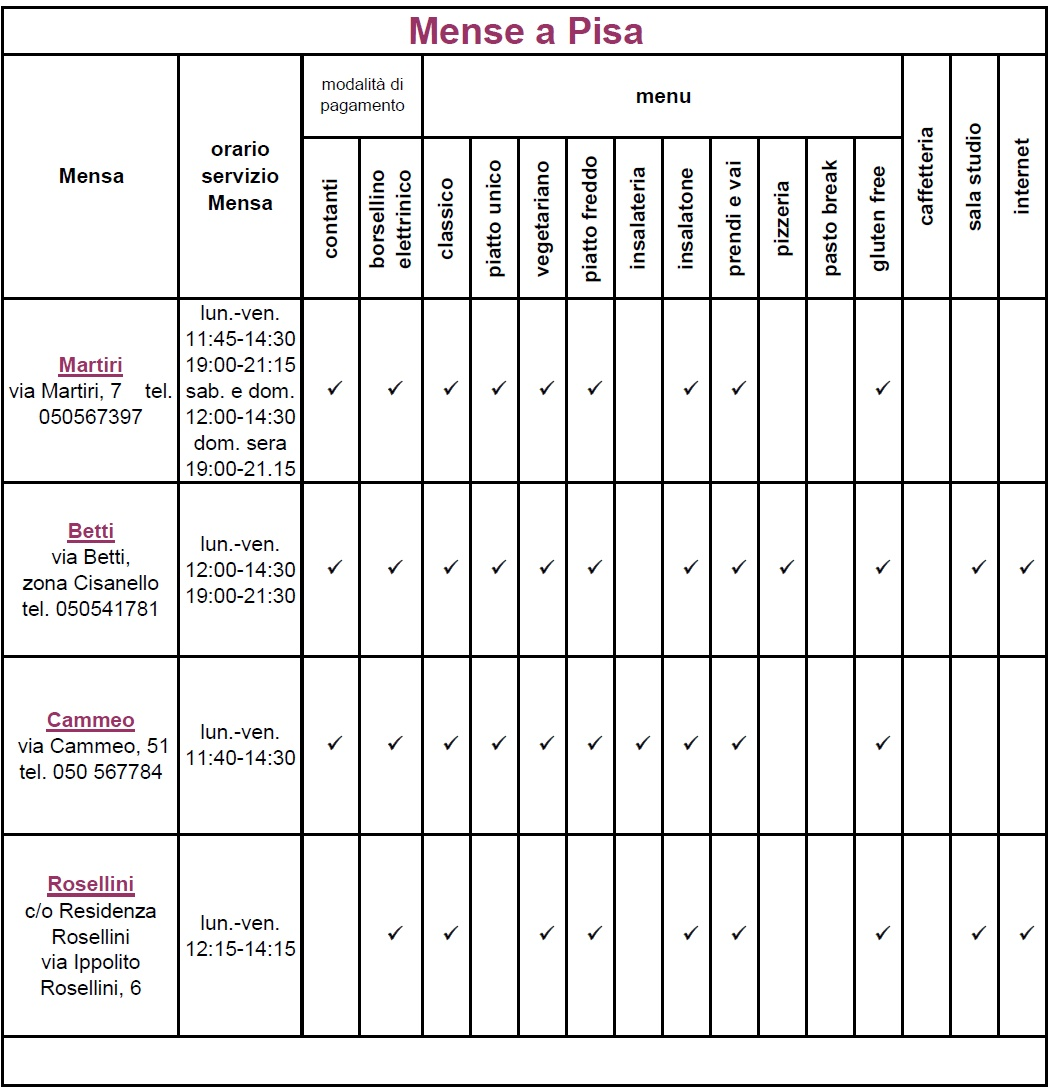
\includegraphics[width=\linewidth]{mense.jpg}\label{fig:mense}
  \caption{University canteens in Pisa. The fifth canteen (not listed here) is inside the residence \textit{I Praticelli} (very close to TeCip institute and CNR area) and it's always open (every day, both for dinner and lunch).}
\end{figure}

%----------------------------------------------------------------------------------------
%	CHAPTER 
%----------------------------------------------------------------------------------------

\chapterimage{ciclopi.png} % Chapter heading image

\chapter{Logistics}

%-----------------------------------------------

\section{Ciclopi}
During your first year, you will surely have to attend a few courses at the Engineering department and at the Computer Science department. To move quickly between these two departments, I strongly recommend getting a bike or getting an account on Ciclopi (bikesharing Pisa) for 25 EUR per year, including 5 EUR credit on the card with no risk of having your bike stolen. Ciclopi lets you get a bike at any of the stalls around the city for free, as long as you return it to any other stall within 30 minutes. The next 30 minutes cost 0.5 EUR. Only warning: some of the bikes are really broken and poorly maintained. In case you buy your own bike, get a strong chain. Me and each one of my peers have very good stories to tell on how our bikes were stolen. 
Visit the official page: \url{http://www.ciclopi.eu}
\begin{figure}[h]
  \centering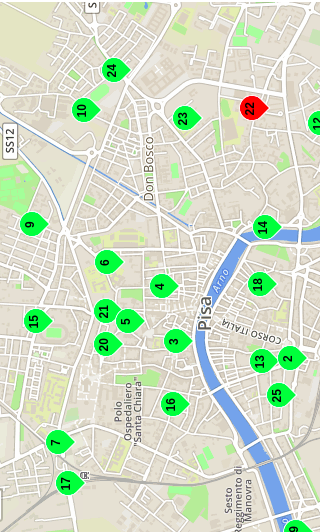
\includegraphics[width=\linewidth]{map_bikes.png}
  \caption{Some of the locations where you can find a CicloPi bike.}
\end{figure}

%-----------------------------------------------

\section{Bus services}
Bus services are also available around the city. The current price for a single (urban) run is 1.50 EUR\footnote{updated: 27th february '19.}.
Visit the official page: \url{http://www.pisa.cttnord.it}
\begin{figure}[h]
  \centering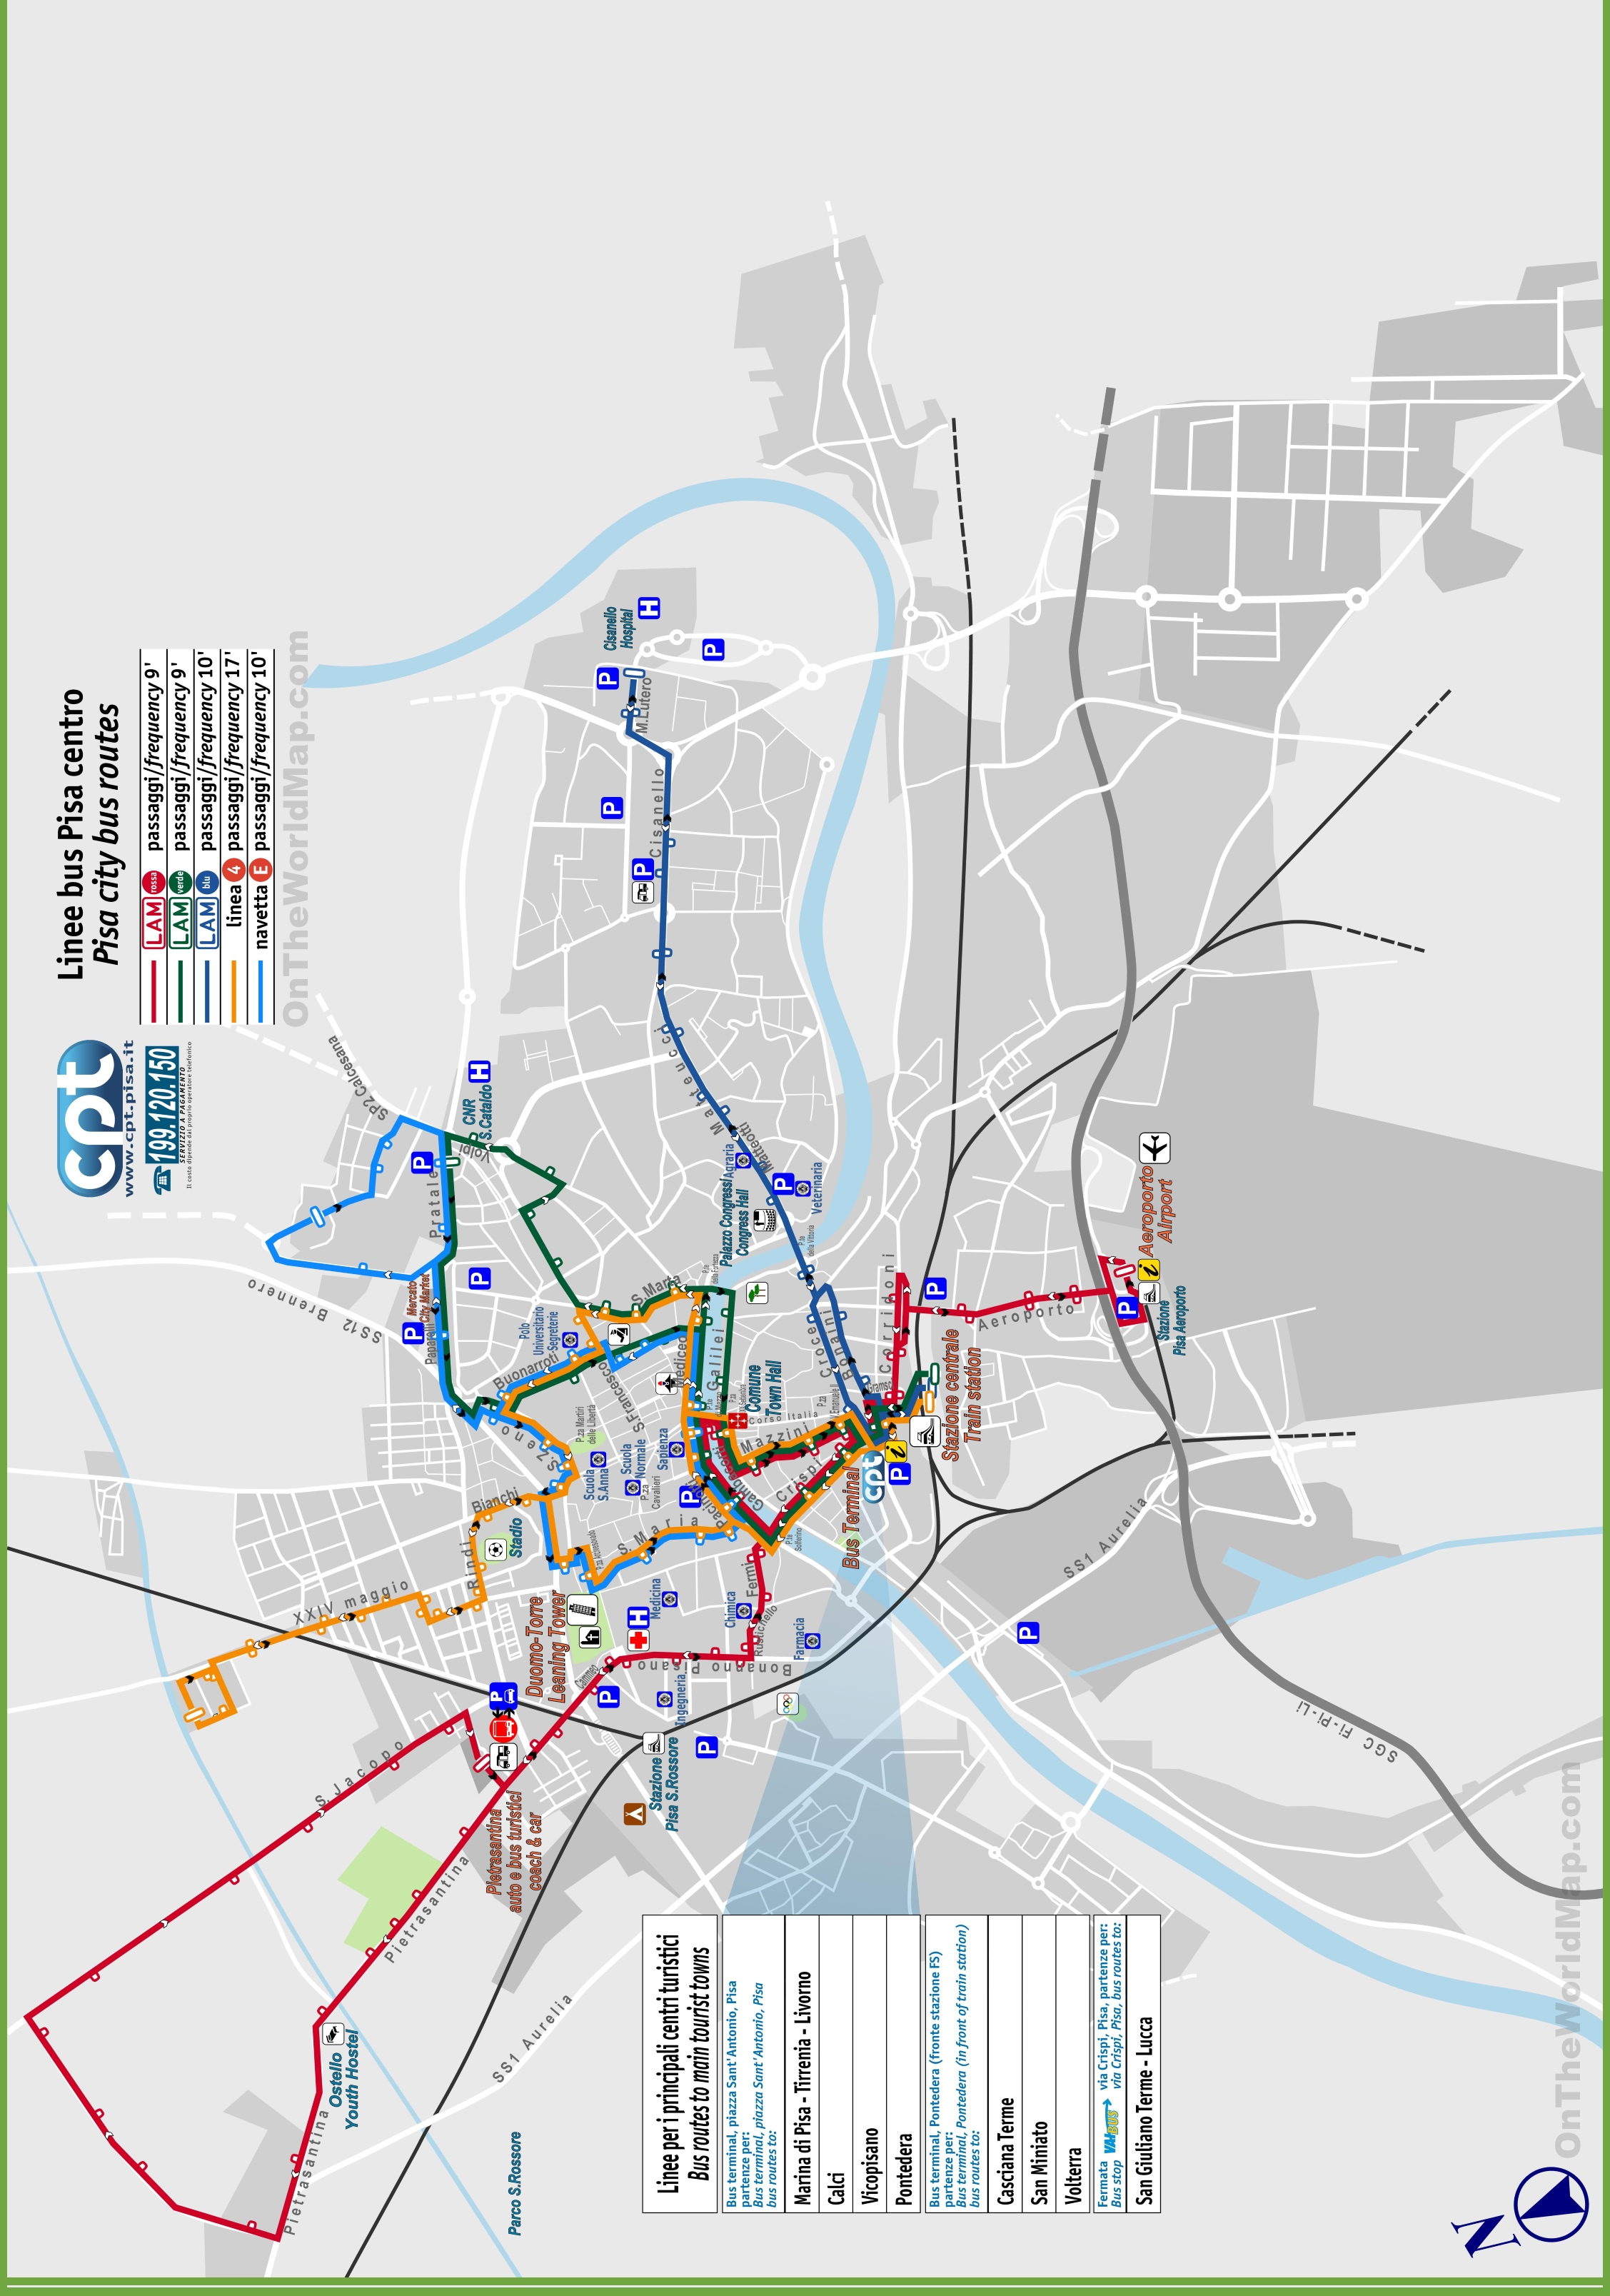
\includegraphics[width=\linewidth]{pisa-bus-routes-map.jpg}
  \caption{The Pisa bus routes map.}
\end{figure}
%----------------------------------------------------------------------------------------
%	CHAPTER 
%----------------------------------------------------------------------------------------

\chapterimage{telephone.jpg} % Chapter heading image

\chapter{Contacts}

%-----------------------------------------------

If you have further questions, we remind you that Prof. Marco Danelutto, the president of the Master’s course, is always available for helping you out! Feel free to ask your student representatives too in case of doubts or if you need further clarifications. We will try to help you as much as possible. 

\paragraph{Some students}\index{Contacts}
\begin{itemize}
\item \textsc{Daniele Gadler} (student representative): daniele.gadler@yahoo.it
\item \textsc{Francesco Tosoni} (student representative): f.tosoni@studenti.unipi.it
\end{itemize}

\end{document}
